\chapter{近似算法}

\begin{introduction}
	\item 近似算法介绍
	\item 顶点覆盖
	\item 任务调度
	\item 最小带权覆盖
	\item MAX-K-SAT
\end{introduction}

本章讲述了NPC问题的一些近似算法及其质量分析。

\section{近似算法介绍}

\subsection{引入与定义}

求解NPC问题的思路通常包括:
\begin{enumerate}
	\item 设计通用的指数级时间复杂度算法
	\item 针对特例设计多项式时间复杂度算法
	\item 根据问题特点设计启发式算法,或借用元启发式算法的框架求解(如蚁群、遗传、退火等算法)
	\item 设计近似算法
\end{enumerate}
其中设计近似算法时便要求时间复杂度是多项式级,得到的解可以保证与最优解比差别有限,具体定义如下。

\begin{definition}{近似算法}{approximation-algorithm:15Ln-ApproximationAlgorithm}
	对一个问题有多项式级时间复杂度,并对任意实例均有$ALG\leqslant \alpha \cdot OPT$,其中$\alpha$为一个常数,则称该算法为此问题的近似算法。(ALG为该算法结果的质量,OPT为最优解的质量)
\end{definition}

\subsection{近似算法常用证明方法}

\begin{figure}[htb]
	\centering
	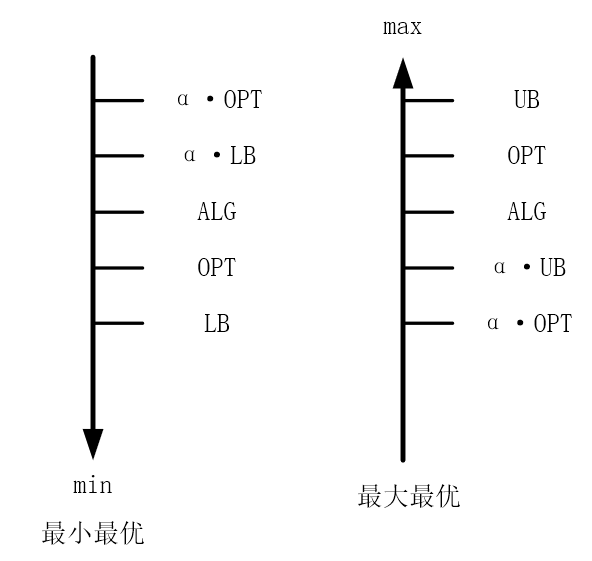
\includegraphics[scale=0.3]{image/Ln15-ApproximationAlgorithm1.png}
	\caption{近似算法证明思路}\label{proof:Ln15-ApproximationAlgorithm}
\end{figure}

\subsubsection{最小最优证明}
一般利用\autoref{proof:Ln15-ApproximationAlgorithm}的证明思路,首先找到OPT下界LB,证明$OPT\geqslant LB$,再想办法证明$ALG\leqslant \alpha \cdot LB$,从而得到$ALG\leqslant \alpha \cdot OPT$,即可证明该近似算法的正确性。
\subsubsection{最大最优证明}
同样利用\autoref{proof:Ln15-ApproximationAlgorithm}的证明思路,首先找到OPT上界UB,证明$OPT\leqslant UB$,再想办法证明$ALG\geqslant \alpha \cdot UB$,从而得到$ALG\geqslant \alpha \cdot OPT$,即可证明该近似算法的正确性。



\section{顶点覆盖}

本节将介绍一个顶点覆盖的近似算法。

\subsection{问题描述}

\begin{definition}{顶点覆盖问题}{vertex-cover:15Ln-ApproximationAlgorithm}
	对于给定的图$(V,E)$,找到一个点集$S\subset V$,使得该图所有边都至少有一个端点在点集S中。
\end{definition}

\subsection{算法描述}

算法步骤如下:
\begin{enumerate}
	\item 找到极大匹配M,相关定义如下:
	\begin{definition}{匹配}{matching:15Ln-ApproximationAlgorithm}
		给定一个图G,在G的一个子图M中,任意两边都没有相同的端点,且每个点都有边相连。
	\end{definition}
	\begin{definition}{极大匹配}{maximal-matching:15Ln-ApproximationAlgorithm}
		一个匹配无法再增加任何点和边,则称之为极大匹配。
	\end{definition}
	\item 输出M中的所有点作为解的点集S
\end{enumerate}

\subsection{正确性证明}

\begin{proposition}{求证}{proof1:15Ln}
该算法始终有$ALG\leqslant 2\cdot OPT$,在该问题中OTP即为最优解点的数量,ALG即为算法求解的点的数量。
\end{proposition}
证明:
\begin{enumerate}
	\item 证明$OPT\geqslant |M|$(其中|M|为极大匹配的边数):对于M中任意一条边,其必定至少有一点在OPT中,否则这条边就未被覆盖,与顶点覆盖的要求矛盾。故$OPT\geqslant |M|$
	\item 证明$ALG=2\cdot |M|$:极大匹配中任意一点度为1,故点的数量即为边的数量的两倍,得证$ALG=2\cdot |M|$。
	\item 根据上述证明可以得到$2\cdot OPT\geqslant 2\cdot|M|=ALG$,得证$ALG\leqslant 2\cdot OPT$
\end{enumerate}
	
\section{任务调度}

\section{最小带权覆盖}

本节将介绍一个最小带权覆盖的近似算法。

\subsection{问题描述}

\begin{definition}{最小带权覆盖问题}{weighted-vertex-cover:15Ln-ApproximationAlgorithm}
	对于给定的图$(V,E)$,各个点有权重w,找到一个点集$S\subset V$,使得该图所有边都至少有一个端点在点集S中,且S中所有点的权重之和比所有可行的解都小。
\end{definition}

\subsection{算法描述}

算法步骤如下:
\begin{enumerate}
	\item 将原问题建模为线性规划问题:原问题是$\forall e=(u,v)\epsilon E$,有$v\epsilon S$或$u\epsilon S$,求$\min \sum_{v\epsilon G} x_vw_v$其中
	\[
		x_v = \begin{cases}
			0 & v\notin S \\
			1 & v\epsilon S
		\end{cases}
	\]\\
	将其转化为线性规划问题,可变为:
	\[
		\begin{cases}
			x_v^*+x_u^*\geqslant 1 			   &\forall e=(u,v)\epsilon E\\
			x_v^*\geqslant 0	   			   &\forall v\epsilon G, x_v\epsilon [0,1]\\
			\min \sum_{v\epsilon G} x_v^*w_v &\forall v\epsilon G\
		\end{cases}
	\]
	\item 使用线性规划求解器求解,再将得到的解转化为原问题的解:
	\[
		x_v=\begin{cases}
			0 &x_v^*<0.5\\
			1 &x_v^*\geqslant 0.5
		\end{cases}
	\]
\end{enumerate}

\subsection{正确性证明}

\begin{proposition}{求证}{proof2:15Ln}
	该算法得到的解是一个顶点覆盖
\end{proposition}
证明:
	因为$\forall e=(u,v)\epsilon E,x_v^*+x_u^*\geqslant 1$,故$x_v^*\geqslant 0.5$或$x_u^*\geqslant 0.5$,故$x_v$和$x_u$至少有一个为1,即至少有一点覆盖该边e。
\begin{proposition}{求证}{proof3:15Ln}
	$ALG\leqslant 2\cdot OPT$
\end{proposition}
证明:
	$OPT\geqslant \sum_{v\epsilon G} x_v^*w_v^*$,而又有$x_v\leqslant 2\cdot x_v^*$,故有
	$ALG=\sum_{v\epsilon G} x_vw_v\leqslant 2\cdot \sum_{v\epsilon G} x_v^*w_v^*\leqslant 2\cdot OPT$,得证。

\section{MAX-K-SAT}

本节将介绍三个MAX-K-SAT的算法。

\subsection{问题描述}

\begin{definition}{K-STA问题}{K-SAT:15Ln-ApproximationAlgorithm}
	对于一个公式F,其由n个子句${C_1,\dot ,C_n}$与运算构成,每个子句又恰好由三个文字或运算构成,即$C_i=L_{i1}\bigvee L_{i2}\bigvee L_{i3}$。求一组文字赋值方案,使得公式F为真。
\end{definition}

\begin{definition}{MAX-K-SAT问题}{max-K-SAT:15Ln-ApproximationAlgorithm}
	对于一个K-SAT问题,求一组赋值方案使得值为真的子句数量最多。
\end{definition}

\subsection{随机算法}

\subsubsection{算法描述}

对所有文字$L_i (i=1,\cdots,n)$等概率随机赋值
\[
	L_i=\begin{cases}
		0 &P=0.5\\
		1 &P=0.5
	\end{cases}
\]

\subsubsection{算法分析}
\begin{itemize}
	\item 易知$P(C_i=1)=1-\frac{1}{2^K} $
	\item 故有$E(ALG)=E(\sum_{i=1}^n C_i)=\sum_{i=1}^n E(C_i)=n\cdot (1-\frac{1}{2^K})$
	\item 又由$ALG\leqslant OTP\leqslant n$
	\item 可得$\frac{E(ALG)}{OPT}\geqslant \frac{E(ALG)}{n}=1-\frac{1}{2^K}\geqslant 0.5$
	\item 注意这里的分子并不是ALG,而是ALG的期望
\end{itemize}

\subsection{确定性贪心算法}

\subsubsection{算法描述}

对于随机算法有该递推式:$E(ALG1)=\frac{1}{2}E(ALG1|L_i=0)+\frac{1}{2}E(ALG1|L_i=1)$。
本算法便基于这一点让本算法的E(ALG2)不小于随机算法的E(ALG1)

\begin{algorithm}
\For{$i=1$\KwTo$n$}{
	\If{$E(ALG1|L_i=0,L_{i-1},\cdots,L_0)>E(ALG1|L_i=1,L_{i-1},\cdots,L_0)$}{$L_i=0$}
	\Else{$L_i=1$}
}
\end{algorithm}

\subsubsection{算法分析}
由算法描述可知,对任何$i=1,\cdots,n$都有
\begin{displaymath}
	E(ALG2|L_{i-1},\cdots,L_0)=max(E(ALG1|L_i=0,L_{i-1},\cdots,L_0),E(ALG1|L_i=1,L_{i-1},\cdots,L_0))	
\end{displaymath}
故有
\begin{displaymath}
E(ALG2)=max(E(ALG1|L_i=0),E(ALG1|L_i=1))\geqslant E(ALG1)
\end{displaymath}

\subsection{线性规划算法}

\subsubsection{算法描述}

在线性规划建模中,记$q_i$为$C_i$的值,$y_i$为$L_i$的值,$f_{ij}$为变元$x_i$在$C_i$中的符号。则变为线性规划问题
\[
	\begin{cases}
		q_i、y_i\epsilon [0,1]\\
		q_i\leqslant \sum _{f_{ij}>0}y_j+\sum _{f_{ij}<0}(1-y_j)\\
		\max \sum_{i=1,\cdots,n}q_i
	\end{cases}
\]
线性规划求解完成后,取
\[
	x_i=\begin{cases}
		1 &P=y_i\\
		0 &P=1-y_i
	\end{cases}
\]

\subsubsection{算法分析}
线性规划求解完成后,对任一子句不妨假设其符号全为正,便于证明推导:
\begin{displaymath}
	\begin{split}
		&\because q_i\leqslant \sum_{j=1,\cdots,K} y_j\\
		&\therefore 1-\frac{q_i}{K}\geqslant \frac{1}{K}\sum_{j=1,\cdots,K}(1-y_j)\ \ \ \ (1)
	\end{split}
\end{displaymath}
故有
\begin{displaymath}
	\begin{split}
		P(C_i=1)&=1-\prod _{j=1}^K(1-y_j)\\
		&\geqslant[\frac{1}{K}\sum_{j=1}^K(1-y_j)]^K\\
		(1)\Rightarrow &\geqslant 1-(1-\frac{q_i}{K})^K\\
		q_i\leqslant 1\Rightarrow &\geqslant q_i[1-(1-\frac{1}{K})^K]\\
		&\geqslant q_i(1-\frac{1}{e})
	\end{split}
\end{displaymath}
故有
\begin{displaymath}
	\begin{split}
		E(ALG)&=E(\sum_{i=1}^n C_i)=\sum_{i=1}^n E(C_i)\\
		&=(1-\frac{1}{e})\sum_{i=1,\cdots,n}q_i\\
		&=(1-\frac{1}{e})*OPT(LP)\\
		&\geqslant(1-\frac{1}{e})OPT
	\end{split}
\end{displaymath}
即$\frac{E(ALG)}{OPT}\geqslant 1-\frac{1}{e}